\chapter{Analyse homepagina: call to actions}
\label{analysehomeappendix}
\textit{3 november 2009} De vier punten op de huidige homepagina van Wakoopa noemen enkel functionaliteit, in plaats van voordelen (\citet{Hoekman2008}) of uniekheid van gebruikers (\citet{Beenen2004}). Door de call-to-actions aan te passen naar een van deze twee uitgangspunten, zou het aantal aanmeldingen (en dus de participatie) moeten verhogen.

\paragraph{huidig:}
\begin{itemize}
    \item{Track your apps\\
      How productive are you?\\
      Know what you use and for how long}

    \item{Discover new software\\
      Our engine recommends you the best web apps and software by looking at your day-to-day usage}

    \item{Share what you use\\
      Make a widget for your site or forum and let everybody know what you love}

    \item{Get updated by friends\\
      What are your buddies or colleagues using? Games? Coding tools? Web apps? Now you know}
\end{itemize}

Naast de bewoording van deze punten, kunnen we ook inhoudelijk kijken naar de punten. Wanneer we de survey bekijken, blijkt dat slechts een derde van de huidige gebruikers wel eens een widget op zijn blog of facebook heeft gezet. Voor het overgrote deel van de gebruikers was dit dus niet een reden om zich aan te melden, en daarmee zijn er wellicht andere functies die bezoekers meer prikkelen. Nieuwe functionaliteit waar huidige gebruikers het meest enthousiast over zijn zijn de aanbevelingen en het web tracking. Deze twee functionaliteiten komen niet duidelijk naar voren. De aanbevelingen worden genoemd, maar slechts indirect, en hetzelfde geld voor web apps.Kijkend naar de enqu\^ete kunnen deze beter prominent in beeld worden gebracht.

Na Web tracking en aanbevelingen zijn de twee grootste nieuwe functionaliteiten waar gebruikers tevreden over zijn het tracken op linux en het reputatie en puntensysteem. Kijkend naar de huidige homepagina staat er nergens op welke platformen wakoopa ge\"installeerd kan worden, en welke worden getrackt. ook het reputatie en puntensysteem wordt niet genoemd, terwijl een significant deel van de gebruikers aangeeft dit een waardevolle toevoeging te vinden.

Met bovenstaande punten kunnen we een nieuw lijstje maken met daarin de functionaliteiten die het belangrijkst zijn en die door huidige gebruikers het meest gewaardeerd worden:
\begin{itemize}
    \item{Track what you use\\
      Keep track of what you use on Windows, Mac OS X, Linux and the web}

    \item{Get recommendations\\
      We analyse your day-to-day usage and recommend you new software}

    \item{Updates from friends\\
      See which applications your friends use and what they think of them}

    \item{Collect awards\\
      Level up to become a Wakoopa overlord and compare with friends}
\end{itemize}

Deze functionele items kunnen we vervolgens omvormen naar een lijst met persoonlijke voordelen, en een lijst met nadruk op de uniekheid van gebruikers:

\paragraph{Voordelen (\citet{Hoekman2008}) }
\begin{itemize}
    \item{Gain insight\\
      Keep track of what you use on Windows, Mac OS X, Linux and the web}

    \item{Find better applications\\
      We analyse your day-to-day usage and recommend you new software}

    \item{Match with friends\\
      See which applications your friends use, what they think of them}

    \item{Become an overlord\\
      Use Wakoopa, get awards and reach the highest level}
\end{itemize}
\paragraph{Uniekheid (\citet{Beenen2004})}
\begin{itemize}
    \item{Find your usage patterns\\
      Keep track of what you use on Windows, Mac OS X, Linux and the web}

    \item{Personal recommendations\\
      We analyse your day-to-day usage and recommend you new software}

    \item{Do you differ from friends?\\
      See which applications your friends use and what they think of them}

    \item{Compete with friends\\
      Use Wakoopa, get awards and become a Wakoopa overlord}
\end{itemize}

    \begin{figure}
      \begin{center}
      \caption{Grafische weergave}
        \subfigure[Origineel]{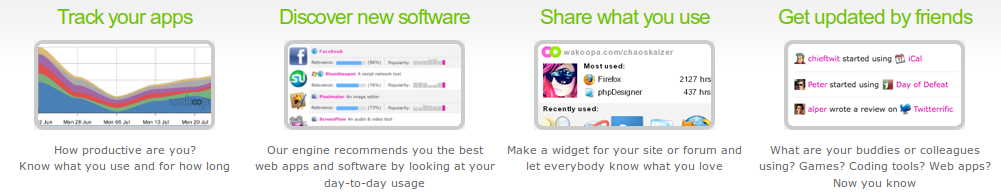
\includegraphics[width=\textwidth]{../images/newhomepage/original}}
        \subfigure[Andere items]{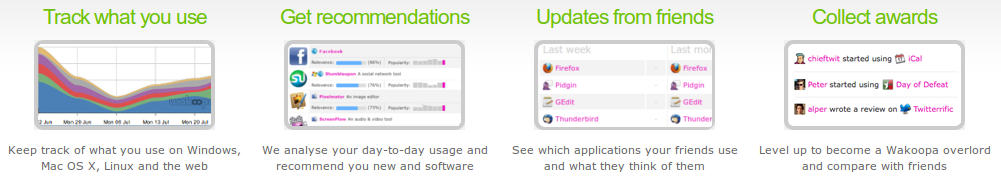
\includegraphics[width=\textwidth]{../images/newhomepage/improved}}
        \subfigure[Voordelen]{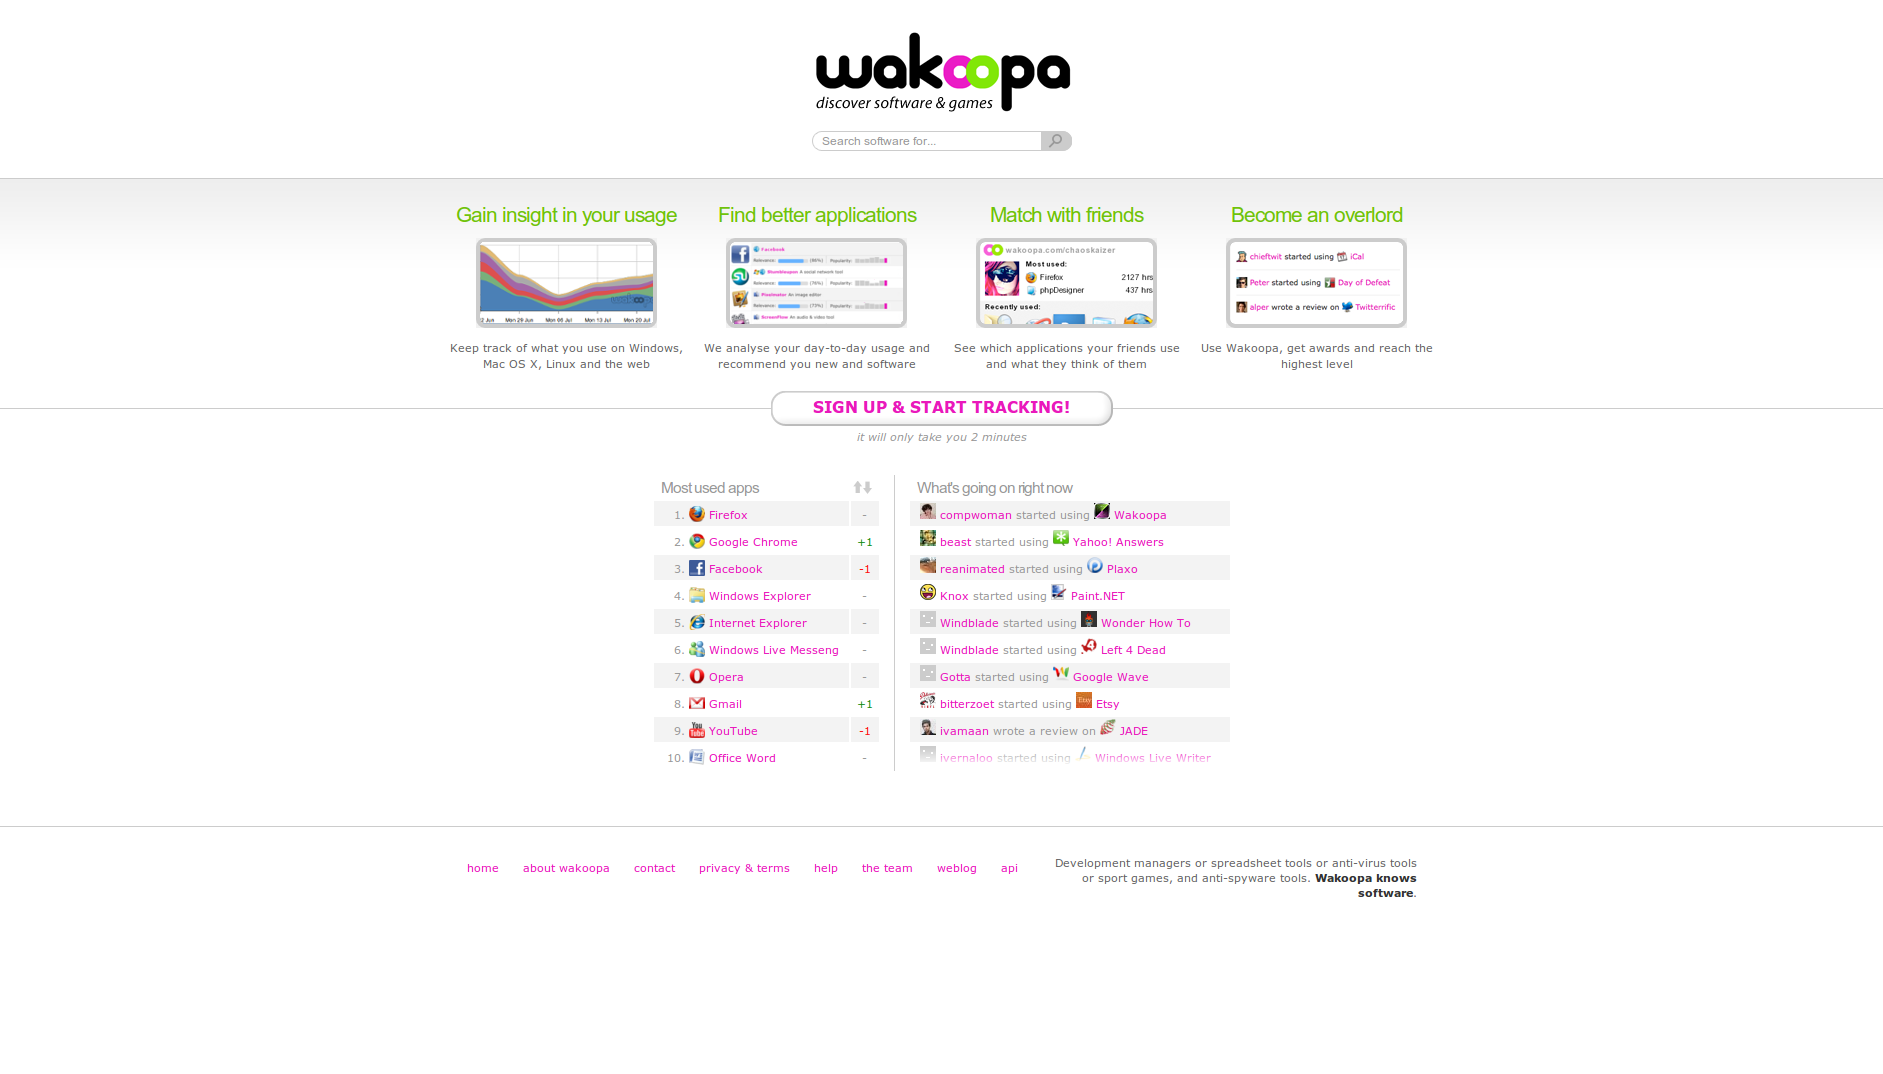
\includegraphics[width=\textwidth]{../images/newhomepage/benefits}}
        \subfigure[Uniekheid]{
\includegraphics[width=\textwidth]{../images/newhomepage/uniqueness}}
      \end{center}
    \end{figure}

